\section{Implementation}
In the previous section we introduced the Alpha algorithm and taken assumptions which were transformed into a timed automaton. The former description should be complete enough to implement Alpha algorithm with any suitable tool of choice. In this section we will focus on implementation with regards to the specific tool of our choice, UPPAAL. As the previous section finished on timed automaton, we will start by presenting timed automaton implemented in UPPAAL. We will draw connections between Figure \ref{fig:automaton} and Figure \ref{fig:automaton_uppaal}. Then we will explain global functions and state. Finally, we will outline the limitations imposed on the model by UPPAAL.

\begin{figure}[H]
\caption{UPPAAL implementation of the automaton}
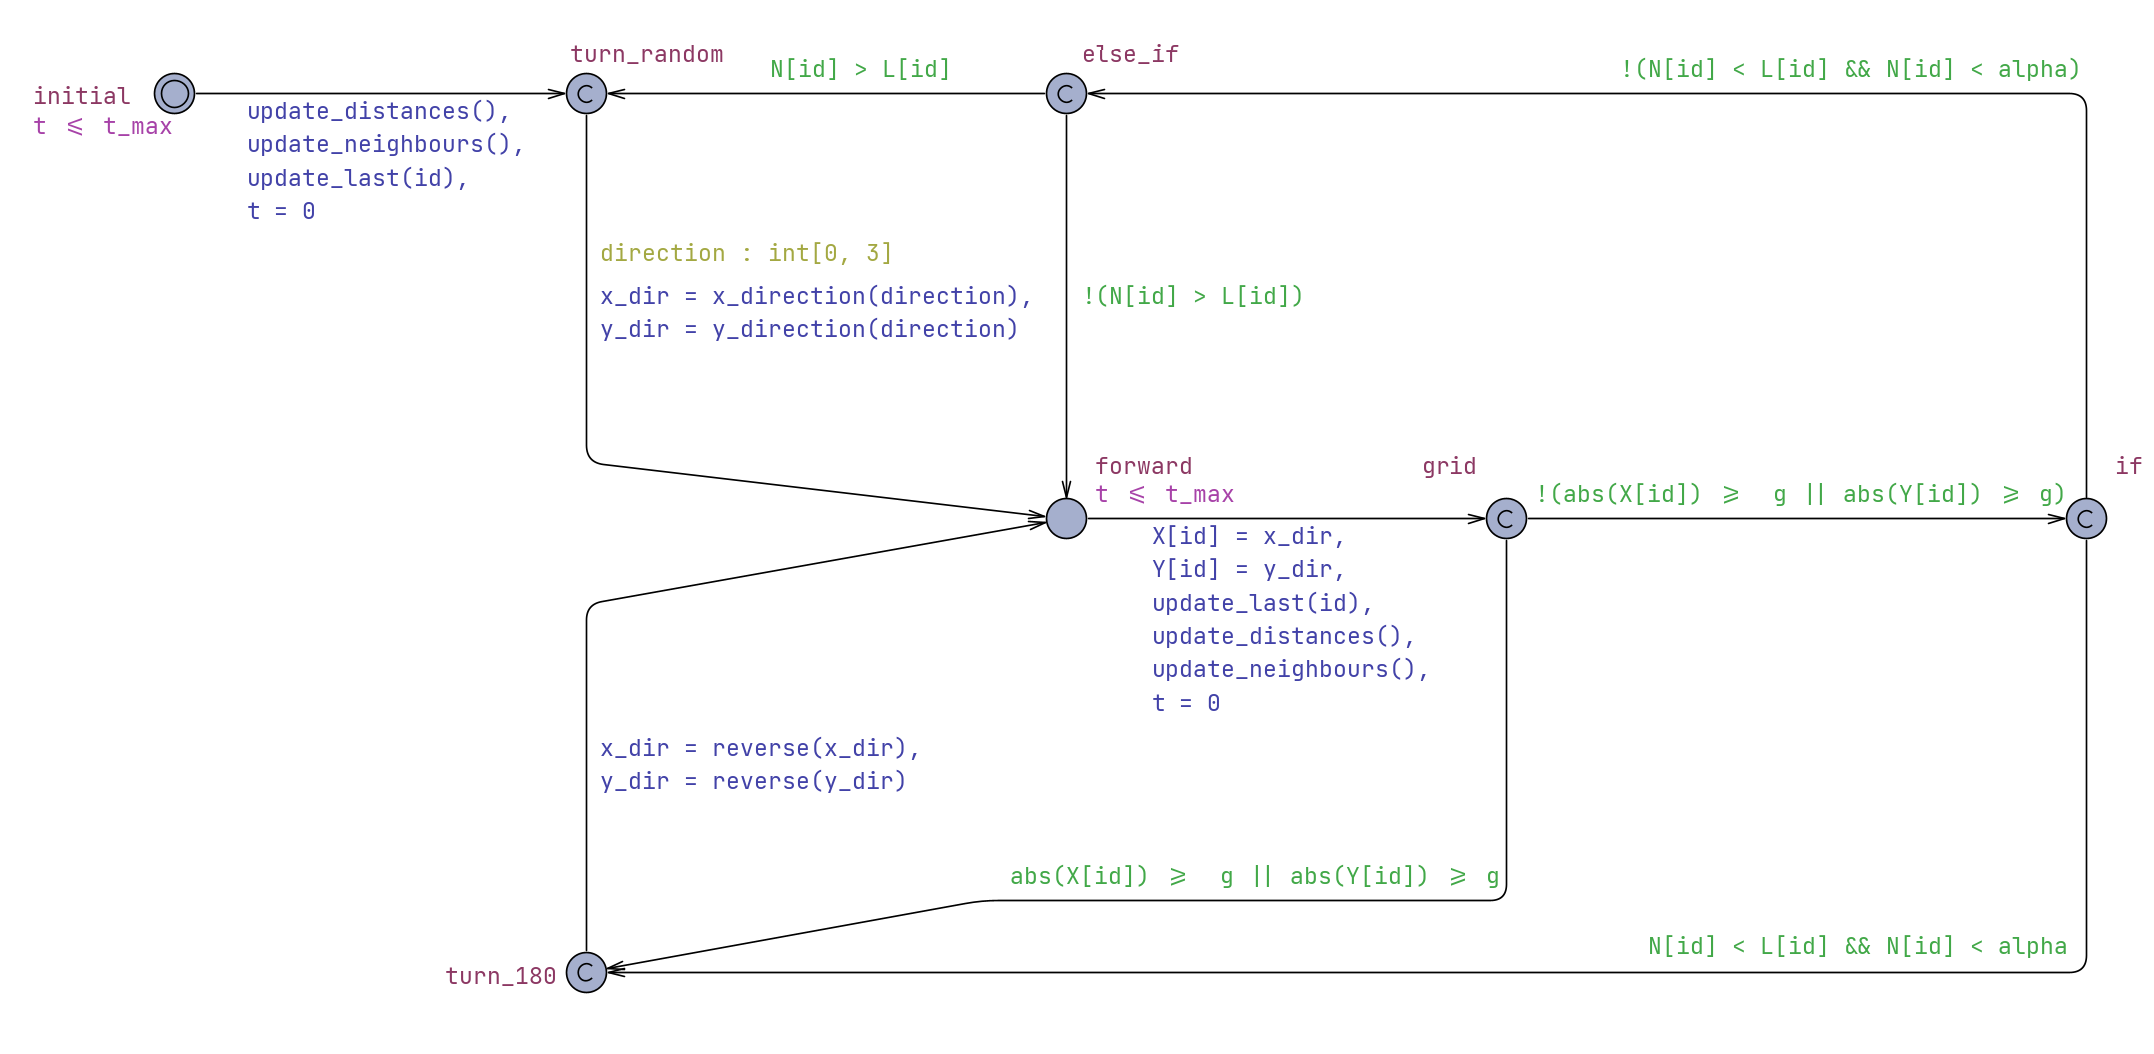
\includegraphics[scale=0.3]{images/automaton_uppaal.png}
\label{fig:automaton_uppaal}
\end{figure}

To start with comparison between general automaton and its specific implementation in UPPAAL, let's notice that both automata have the same set of states and transitions. Guarded transitions use the same conditions. Each robot accesses its own set of condition variables by providing \textbf{id} to the global arrays. Array \textbf{N} holds the number of neighbours for each robot. Array \textbf{L} holds the last number of neighbours for each robot. Those variables are held in the global arrays so that a single robot could update the number of neighbours for all of the other robots when it moves. It may seem counter intuitive that a single robot updates the variables of other robots. However, the execution of the system composed from multiple robots is based on interleaving. At any given time a single robot transitions between states. This means that only the moving robot is guaranteed to have true information about number connections. Global updates of number of neighbours is a way to mimic physical, continuous signal that would determine whether robots are connected or not. It eliminates the situation where robot would make a decision on already outdated information. Implementation assumes that each time a robot moves it will update its coordinates, update the last number of neighbours for itself and update the current number of neighbours for all robots. It achieves the last two actions by calling \textbf{update\_last(id)} and \textbf{update\_neighbours()}. Figure \ref{fig:neighbours} shows the process of updating the number of connections for all robots.
\begin{figure}[H]
\caption{Implementation of \textbf{update\_neighbours()} and \textbf{neighbours()}}
\lstset { language=C++ }
\begin{lstlisting}
int neighbours(int id){
    // returns the number of connections for a robot with a given id
    int x = X[id];  // x coordinate
    int y = Y[id];  // y coordinate
    int k = 0;      // neighbour counter k
    int i = 0;   
    for (i = 0; i < n; i++){
        double d = distance(x, y, X[i], Y[i]);
        bool c = connected(d);
        // is robot connected to another robot
        if(i != id && c){
            k++;
        }
    }
    return k;
}

void update_neighbours(){
    // updates the array that stores number of neighbours for each robot
    int i;
    for (i = 0; i < n; i++){
        N[i] = neighbours(i);
    }
}
\end{lstlisting}
\label{fig:neighbours}
\end{figure}